\section{Aplicaciones}
En esta capa se encuentran las aplicaciones usadas por los usuarios de la red. 

Los \textbf{procesos} (programas) que se ejecutan en un mismo host se pueden comunicar entre sí usando los sistemas de comunicación interproceso definidos por el sistema operativo sobre el que están corriendo.

Cuando un proceso necesita comunicarse con procesos ejecutándose en otros hosts, debe hacerlo usando algún protocolo de la capa de aplicación. Esto protocolos definen mensajes, reglas, acciones y servicios que deben aceptar las aplicaciones en cada punta de la conexión para poder comunicarse y hace uso de la capa de transporte para lograrlo.

\subsection{Modelo Cliente-Servidor}
En este modelo, un proceso cliente inicia la comunicación con un proceso servidor. El servidor espera a que lleguen conexiones de clientes y cuando llega una, la acepta y responde al cliente con los recursos solicitados.

Para identificar un proceso en un host se utiliza un \textbf{socket} que es un número formado por la dirección IP de un host y un número \textbf{port} que identifica el proceso dentro del host. 

Cuando el paquete que desea enviar la aplicación llega a la capa de transporte, se utiliza TCP o UDP (dependiendo del protocolo de aplicación elegido) para enviar el mensaje al destino. La elección del protocolo de transporte depende de la aplicación y de las características de la red. 

\subsection{Domain Name System (DNS)}
Es un servicio de resolución de nombres jerárquico distribuido. Se utiliza para traducir nombres de hosts a direcciones IP. Está implementado como un sistema de bases de datos distribuido generalizado para almacenar una variedad de información relacionada con la elección de un nombre.

Cuando un proceso necesita comunicarse con una llama a un procedimiento llamado \textbf{resolvedor} y le pasa como parámetro el nombre del host con el que desea comunicarse, por ejemplo: "www.google.com". El resolvedor envía un paquete UDP a un servidor DNS local que tiene configurado en el sistema. Este servidor devuelve la dirección IP correspondiente al servidor local y el último lo devuelve al host que originó el pedido.

Una vez que el host conoce la dirección IP del servidor, puede iniciar la comunicación con él usando UDP o TCP.

\subsubsection{Espacio de dominios}
La Internet está dividida en más de 250 \textbf{dominio de nivel superior} (Top-Level Domain), donde cada dominio cubre muchos hosts. Cada dominio está particionado en subdominios, y estos son particionados aún más, y así sucesivamente. Todos estos dominios pueden ser representados por un arbol, donde cada nodo interno es un dominio o subdominio y cada hoja es un host.

\begin{figure}[H]
	\centering
	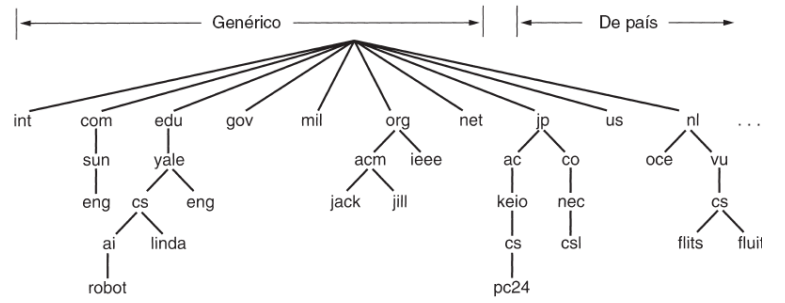
\includegraphics[width=\textwidth
]{images/dns-tree.png}
	\caption[Arbol de dominios DNS]{Arbol de dominios DNS}
	\label{fig:dns-tree}
\end{figure}

Los dominios de nivel superior vienen en dos sabores: genéricos y países.  Los dominios genéricos incluyen dominios originales de los 80s y dominios introducidos a través de aplicaciones a ICANN. Otros dominios de nivel superior genéricos serán agregados en el futuro.

Obtener un dominio de segundo nivel, como nombre-de-empresa.com, es fácil. Los dominios de nivel superior son administrados por registradores designados por la \textbf{Internet Corporation for Assigned  names and Numbers} (ICANN). Obtener un nombre simplemente requiere ir a un registrador correspondiente (para com en este caso) para verificar si el nombre deseado está disponible y no es una marca registrada de otra persona. Si no hay problemas, el solicitante paga al registrador una pequeña tarifa anual y obtiene el nombre.

\subsubsection{Registros DNS}
Cada dominio, ya sea un único host o un dominio de nivel superior, puede tener un conjunto de registros de recursos asociados con él. Estos registros son la base de datos DNS. Para un único host, el registro de recursos más común es solo su dirección IP, pero también existen muchos otros tipos de registros de recursos. Cuando un resolvedor le da un nombre de dominio a DNS, lo que obtiene son los registros de recursos asociados con ese nombre. Por lo tanto, la función principal de DNS es asignar nombres de dominio a registros de recursos.

Un registro de recursos es una tupla de cinco. Aunque están codificados en binario para la eficiencia, en la mayoría de las exposiciones los registros de recursos se presentan como texto ASCII, una línea por registro de recursos.

\[< \texttt{nombre\_dominio}, \texttt{tiempo\_de\_vida}, \texttt{clase}, \texttt{tipo}, \texttt{valor},>\]

\begin{itemize}
  \item El \textbf{nombre\_dominio} es el nombre de dominio asociado al registro de recursos.
  \item El \textbf{tiempo\_de\_vida} indica que tan estable es el registro. Información que se actualiza periódicamente tiene un tiempo de vida corto, mientras que información que cambia raramente tiene un tiempo de vida largo.
  \item La \textbf{clase} es siempre IN, que significa Internet. Hay otras clases de recursos, pero no se usan en la práctica.
  \item El campo \textbf{tipo} indica el tipo de recursao y el campo \textbf{valor} contiene la información correspondiente y significa distintas cosas dependiendeo del tipo de recurso:
  \begin{itemize}
    \item \textbf{SOA} (Start of Authority): Información sobre el servidor de la zona, el administrador, timeouts y como esta configurado
    \item \textbf{A} (Address): Dirección IP de un host que acepta mensajes en el dominio.
    \item \textbf{MX} (Mail Exchange): Nombre de algún host dentro del dominio que acepta emails.
    \item \textbf{NS} (Name Server): Nombre de un servidor DNS dentro del dominio.
    \item \textbf{CNAME} (Canonical Name): Nombre canónico de un alias, se utiliza cuando el dominio consultado en realidad es un alias de otro dominio
    \item \textbf{PTR} (Pointer): Nombre de dominio asociado a una dirección IP específica.
    \item \textbf{HINFO} (Host Information): Información sobre el host, como el tipo de CPU y el sistema operativo.
    \item \textbf{TXT} (Text): Texto arbitrario asociado con el nombre de dominio.
  \end{itemize}
\end{itemize}

\subsubsection{Resolución de nombres}
En teoría, un solo servidor de nombres podría contener toda la base de datos de DNS y responder a todas las consultas sobre ella. En la práctica, este servidor estaría tan sobrecargado como para ser útil. Además, si alguna vez se cae, toda la Internet se vería afectada.

Para evitar los problemas asociados con tener una sola fuente de información, el espacio de nombres de DNS se divide en zonas no superpuestas. Cada zona está asociada con uno o más servidores DNS que contienen la base de datos de la misma. Normalmente, una zona tendrá un DNS primario, que obtiene su información de un archivo en su disco, y uno o más DNS secundarios, que obtienen su información del DNS primario. 

El proceso de buscar un nombre y encontrar una dirección se llama \textbf{resolución de nombres}. Cuando un resolvedor tiene una consulta sobre un nombre de dominio, pasa la consulta a un DNS. Si el dominio que se busca está bajo la jurisdicción del mismo, el DNS local responde con la dirección IP correspondiente. Si el dominio no está bajo la jurisdicción su jurisdicción, el DNS pasa la consulta a un un DNS de nivel superior.

El DNS de nivel superior responde con la dirección IP del DNS de la zona que contiene el dominio buscado. El servidor de DNS local luego pasa la consulta al DNS de la zona, que responde con la dirección IP del dominio buscado. Finalmente, el DNS local pasa la dirección IP al resolvedor, que puede entonces iniciar la comunicación con el host.

\begin{figure}[H]
	\centering
	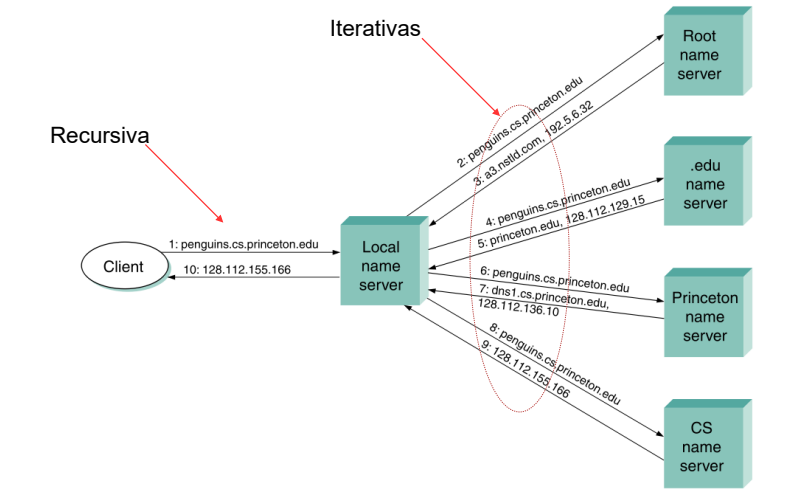
\includegraphics[width=0.8\textwidth
]{images/dns-queries.png}
	\caption[Consulta DNS]{Consulta DNS}
	\label{fig:dns-queries}
\end{figure}

Si el dominio que se busca está bajo la jurisdicción del DNS, se dice que la respuesta obtenida es \textbf{autoritativa}:  Un \textbf{registro autoritativo} es aquel que proviene de la autoridad que administra el registro y, por lo tanto, siempre es correcto. Las respuestas no autoritativas son respuestas que no provienen de la autoridad que administra el registro y, por lo tanto, pueden estar desactualizadas.

%Traducir:
If the domain being sought falls under the jurisdiction of the  
name server, such as top.cs.vu.nl falling under cs.vu.nl, it returns the authoritative  
resource records. An authoritative record is one that comes from the authority  
that manages the record and is thus always correct. Authoritative records are in  
contrast to cached records, which may be out of date 
%A español:
Si el dominio que se busca está bajo la jurisdicción del servidor de nombres, como top.cs.vu.nl que cae bajo cs.vu.nl, devuelve los registros de recursos autoritativos. Un registro autoritativo es aquel que proviene de la autoridad que administra el registro y, por lo tanto, siempre es correcto. Los registros autoritativos están en contraste con los registros en caché, que pueden estar desactualizados.

\subsection{Envío de correo electrónico (SMTP)}
\subsubsection{Agente de usuarios:}
El agente de usuario es un programa que proporciona una interfaz gráfica, o a veces una interfaz basada en texto y comandos que permite a los usuarios interactuar con el sistema de correo electrónico. Incluye un medio para componer, responder, mostrar y organizar mensajes. El acto de enviar nuevos mensajes al sistema de correo para su entrega se llama envío de correo.

Después de que se ha leído un mensaje, el usuario puede decidir qué hacer con él. Esto se llama disposición del mensaje. Las opciones incluyen eliminar el mensaje, enviar una respuesta, reenviar el mensaje a otro usuario y guardar el mensaje para referencia posterior. La mayoría de los agentes de usuario pueden administrar un buzón para correo entrante con varias carpetas para correo guardado. Las carpetas permiten al usuario guardar el mensaje según el remitente, el tema u otra categoría.

\subsubsection{Servidor de correo}
Los agentes de transferencia de mensajes son procesos del sistema. Se ejecutan en segundo plano en las máquinas del servidor de correo y están destinados a estar siempre disponibles. Su trabajo es mover automáticamente el correo electrónico a través del sistema desde el remitente hasta el destinatario con SMTP (Protocolo simple de transferencia de correo). Este es el paso de transferencia de mensajes.

\subsubsection{Formato de email}
El encabezado contiene toda la información necesaria para transportar el mensaje, como la dirección de destino, la prioridad y el nivel de seguridad, todos los cuales son distintos del mensaje en sí. Los agentes de transporte de mensajes utilizan esta información para el enrutamiento. Los campos más relevantes del encabezado son:
\begin{center}
  \begin{tabularx}{0.8\textwidth}{l|p{0.6\textwidth}}
    \textbf{Campo} & \textbf{Descripción} \\
    \hline
    To & Direcciónes de correo de los destinatarios primarios \\
    CC & Direcciónes de correo de los destinatarios secundarios \\
    BCC & Direcciónes de correo de los destinatarios ocultos \\
    From & Persona o personas que crearon el mensaje \\
    Sender & Dirección de correo del remitente \\
    Received & Lista de servidores de correo que han recibido el mensaje \\
    Return-Path & Usado por el servidor para identificar una ruta de regreso al remitente \\
    Date & Fecha y hora en que se envió el mensaje \\
    Reply-To & Dirección de correo a la que se debe responder \\
    Message-Id & Identificador único para el mensaje \\
    In-Reply-To & Identificador único para el mensaje al que se está respondiendo \\
    References & Identificadores únicos para mensajes relacionados \\
    Keywords & Palabras clave para ayudar a los usuarios a encontrar el mensaje \\
    Subject & Tema del mensaje \\
  \end{tabularx}
\end{center}

\newpage
\subsubsection*{MIME - Multipurpose Internet Mail Extensions}
MIME define cinco nuevos encabezados de mensajes:
\begin{itemize}
  \item \textbf{MIME-Version}: Incidica al agente de usuario que recibe el mensaje que está tratando con un mensaje MIME y qué versión de MIME usa. Cualquier mensaje que no contenga un encabezado MIME-Version: se asume que es un mensaje de texto en inglés (o al menos uno que usa solo caracteres ASCII) y se procesa como tal.
  \item \textbf{Content-Description}: Proporciona una descripción en inglés del contenido del mensaje.
  \item \textbf{Content-Id}: Proporciona un identificador único para el contenido del mensaje.
  \item \textbf{Content-Transfer-Encoding}: Indica cómo se codificó el contenido para que se pueda transmitir a través de la red. 
  
  La codificación más usada se llama \textbf{base64 encoding}. En este esquema, grupos de 24 bits se dividen en cuatro unidades de 6 bits, y cada unidad se envía como un carácter ASCII legal. Para mensajes que son casi completamente ASCII pero con algunos caracteres no ASCII, se utiliza un esquema de codificación conocido como \textbf{quoted-printable encoding}.

  Finalmente, cuando hay razones válidas para no usar uno de estos esquemas, es posible especificar una codificación definida por el usuario.
  
  \item \textbf{Content-Type}: Indica el tipo de contenido que contiene el mmensaje:
  \begin{center}
    \begin{tabularx}{0.8\textwidth}{l|l|l}
      \textbf{Tipo} & \textbf{Ejemplos de Subtipo} & \textbf{Descripción} \\
      \hline
      text & plain, html, xml, css & Texto plano en varios formato \\
      image & gif, jpeg, tiff & Imagenes \\
      audio & basic, mpeg, mp4 & Audio \\
      video & mpeg, mp4, quicktime & Video MPEG \\
      model & vrml & Modelos 3D \\
      application & octet-stream, pdf, js, zip & Datos producidos por aplicaciones \\
      message & http, rvf822 & Mesnaje encapsulado \\
      multipart & mixed, alternative, parallel, digest & Combinación de varios tipos \\
    \end{tabularx} 
  \end{center}
\end{itemize}

\subsubsection*{Transferencia de mensajes}
El correo electrónico se entrega haciendo que la computadora de envío establezca una conexión TCP al puerto 25 de la computadora de recepción. Escuchando este puerto hay un servidor de correo que habla SMTP (Protocolo simple de transferencia de correo). Este servidor acepta conexiones entrantes, sujeto a algunas verificaciones de seguridad, y acepta mensajes para su entrega. Si un mensaje no se puede entregar, se devuelve un informe de error que contiene la primera parte del mensaje no entregable al remitente.

Una vez que el servidor SMTP recibe un mensaje del agente de usuario, lo entregará al servidor SMTP que corresponde a la dirección del remitente del mail. Para identificar este servidor se utiliza una consulta DNS, se crea una conexión TCP entre ambos servidores parar transferir el mensaje usando SMTP y luego se cierra la conexión.

Cuando el usuario remitente quiera leer su correo, el agente de usuario se conecta al servidor de correo de recepción usando POP3 (Protocolo de oficina de correos versión 3) o IMAP (Protocolo de acceso a mensajes de Internet).

\subsubsection*{IMAP - Internet Message Access Protocol}
Uno fde los protocolos más usados en para realizar el delivery final al remitente es IMAP:

El cliente inicia un conexión seguro al servidor de mails y luego inicia sesión o se autentique de algun manera. Una vez iniciada la sesión, hay muchos comandos para enumerar carpetas y mensajes, recuperar mensajes o incluso partes de mensajes, marcar mensajes con banderas para su eliminación posterior y organizar mensajes en varias badnejas de entrada.

IAMP es un mejor de POP3, un protocolo más simple y menos seguro en el cual cada mail se descargaba en la computadora del usuario, en vez de mantenerse en los servidores de mail. 

\paragraph{Resumen IMAP y POP3}
\begin{center}
  \begin{tabularx}{0.8\textwidth}{l|l|l}
    \textbf{Característica} & \textbf{POP3} & \textbf{IMAP} \\
    \hline
    En dónde se define el protocolo & RFC 1939 & RFC 2060 \\
    \hline
    Puerto TCP utilizado & 110 & 143 \\
    \hline
    En donde se almacena el email & PC del usuario & Servidor \\
    Como se lee el correo electrónico  & Sin conexión & \\
    Tiempo de conexión requerido & Breve & Largo \\
    \hline
    Uso de recursos de servidor & Bajo & Alto \\
    \hline
    Múltiples buzones de entrada & No & Si \\
    \hline
    Quien resplalda los buzones & Usuario & Servidor \\
    \hline
    Bueno para los usarios moviles & No & Si \\
    \hline
    Control del usuario sobre la descarga & Poco & Mucho \\
    \hline
    Descargas parciales de mensajes & No & Si \\
    Sencillo de implementar & Si & No \\
    \hline
    Soporte amplio & Si & No \\
  \end{tabularx}
\end{center}

\subsection{HTTP: Hypertext Transfer Protocol}
Desde el punto de vista de los usuarios, la Web consiste en una vasta colección mundial de contenido en forma de páginas web. Cada página puede contener enlaces a otras en cualquier parte del mundo. Los usuarios pueden seguir un enlace haciendo clic en él, lo que los lleva a la página a la que apunta. La idea de tener una página que apunte a otra es llamada \textbf{hipertexto}. Un pedazo de texto, icono, imagen, etc. asociado con otra página se llama \textbf{hipervínculo}.

Cada página se obtiene enviando una solicitud a uno o más servidores, que responden con el contenido de la página. El protocolo de solicitud-respuesta para obtener páginas es un protocolo de texto simple que se ejecuta sobre TCP, tal como era el caso de SMTP. Se llama \textbf{HTTP (Protocolo de transferencia de hipertexto)}. El contenido puede ser simplemente un documento que se lee de un disco, o el resultado de una consulta a una base de datos y la ejecución de un programa. La página es una \textbf{página estática} si es un documento que es el mismo cada vez que se muestra. En contraste, si se generó a pedido por un programa o contiene un programa, es una \textbf{página dinámica}.

Cada página se le asigna una \textbf{URL (Localizador de recursos uniforme)} que efectivamente sirve como el nombre mundial de la página. Las URL tienen tres partes: el protocolo (también conocido como el esquema), el nombre DNS de la máquina en la que se encuentra la página y la ruta que indica de forma única la página específica (un archivo para leer o programa para ejecutar en la máquina). En el caso general, la ruta tiene un nombre jerárquico que modela una estructura de directorio de archivos.

Cuando un usuario hace clic en un hipervínculo, el navegador realiza una serie de pasos para buscar la página a la que apunta:
\begin{enumerate}
  \item El navegador determina la URL (viendo lo que se seleccionó).
  \item El navegador hace una consulta DNS, la dirección IP del servidor donde está la página guardada.
  \item El navegador establece una conexión TCP con el servidor en el puerto 80, el puerto conocido para el protocolo HTTP.
  \item El navegador envía una solicitud HTTP pidiendo la página /index.html.
  \item El servidor envía la página solicitada.
  \item Si la página contiene hipervínculos, el navegador repite el proceso para cada uno de ellos usando la misma conexión TCP.
  \item En HTTP1.0 la conexión se cierra y el navegador debe volver a realizar todos los pasos anteriores para pedir un nuevo recuro. En HTTP 2.0, la conexión TCP se mantiene abierta mientras el navegador sigue pidiendo recursos y se cierra despues de un tiempo de que se deja usar.
\end{enumerate}

\subsubsection{Cookies}
Navegar por la Web como lo hemos descrito hasta ahora implica una serie de recuperaciones de páginas independientes. No hay concepto de una sesión de inicio de sesión. El navegador envía una solicitud a un servidor y recibe un archivo. Luego, el servidor olvida que alguna vez ha visto a ese cliente en particular.

Este problema se resuelve con un mecanismo a menudo criticado llamado cookies.

Cuando un cliente solicita una página web, el servidor puede proporcionar información adicional en forma de una cookie junto con la página solicitada. La cookie es una cadena de nombre pequeño (de como máximo 4 KB) que el servidor puede asociar con un navegador.

Esta asociación no es lo mismo que un usuario, pero es mucho más cercana y útil que una dirección IP. Los navegadores almacenan las cookies ofrecidas durante un intervalo, generalmente en un directorio de cookies en el disco del cliente para que las cookies persistan a través de las invocaciones del navegador, a menos que el usuario haya desactivado las cookies. Las cookies son solo cadenas, no programas ejecutables. En principio, una cookie podría contener un virus, pero dado que las cookies se tratan como datos, no hay una forma oficial para que el virus se ejecute y cause daños. Sin embargo, siempre es posible que algún hacker explote un error del navegador para causar la activación.

Una cookie puede contener hasta cinco campos:
\begin{itemize}
  \item \textbf{Dominio:} El dominio indica a que sitio web pertenece la cookie.
  \item \textbf{Ruta:} La ruta indica a que directorio pertenece la cookie.
  \item \textbf{Content:} El contenido es un diccionario de de clave, valor separados por un signo igual.
  \item \textbf{Fecha de expiración:} La fecha de expiración indica cuando la cookie debe ser eliminada. Si este campo está ausente, entonces se dice que es una \textbf{cookie persistente}. Sino, es una \textbf{cookie no persistente}.
  \item \textbf{Secure:} Indica si la cookie debe ser enviada solo a través de conexiones seguras.
\end{itemize}

\subsubsection{Mensajes HTTP}

Aunque HTTP fue diseñado para su uso en la Web, se hizo intencionalmente más general de lo necesario con miras a futuros usos orientados a objetos. Por esta razón, se admiten operaciones, llamadas métodos, que no solo solicitan una página web:

\begin{itemize}
  \item \textbf{GET:} El cliente solicita un objeto y el servidor responde con el objeto solicitado o un mensaje de error.
  \item \textbf{HEAD:} Se usa cuando, al cliente, solo le interesa la información contenida en el header de la respuesta. El servidor no envía el objeto, solo el encabezado.
  \item \textbf{POST:} El cliente envía un objeto al servidor y el último usa este objeto para realizar alguna acción, por ejemplo, modificar una base de datos, comprar algún item o ejecutar algún programa. El servidor responde con una página indicando el resultado de la operación realizada.
  \item \textbf{PUT:} Se usa para modifciar algún objeto ya guardado en servidor.
  \item \textbf{DELETE:} Se usa para eliminar algún objeto guardado en el servidor.
  \item \textbf{TRACE:} Se usa para que el servidor devuelva el mensaje recibido, esto se usa para debuggear.
  \item \textbf{OPTIONS:} Se usa para que el servidor devuelva los métodos que soporta.
  \item \textbf{CONNECT:} Se usa para establecer un túnel TCP/IP con el servidor.
\end{itemize}

Todas las respuestas están formadas por un header y un body. El header contiene información sobre la respuesta y el body contiene el objeto solicitado. El header contiene los siguientes campos:

\begin{itemize}
  \item \textbf{Status line:} Contiene el protocolo, la versión y el código de estado de la respuesta. El código de estado es un número de tres dígitos que indica el resultado de la operación:
  \begin{center}
    \begin{tabularx}{0.8\textwidth}{l|l|l}
      \textbf{Código} & \textbf{Descripción} & \textbf{Ejemplo} \\
      \hline
      1xx & Información & 100 Continue \\
      2xx & Éxito & 200 OK \\
      3xx & Redirección & 301 Moved Permanently \\
      4xx & Error del cliente & 404 Not Found \\
      5xx & Error del servidor & 500 Internal Server Error \\     
    \end{tabularx}
  \end{center}
  \item \textbf{User-Agent:} Indica el nombre del navegador que realizó la solicitud.
  \item \textbf{Content-Type:} Indica el tipo de contenido del cuerpo del mensaje.
  \item \textbf{Accept:} Indica los tipos de contenido que acepta el cliente.
  \item \textbf{If Modified Since:} Indica la fecha de la última modificación del objeto solicitado.
  \item \textbf{Host:} Indica el nombre del host al que se le está haciendo la solicitud.
  \item \textbf{Authorization:} Es necesario para páginas que están protegidas. En este caso, el usuario debe probar que tiene las credenciales necesarias para realizar las operaciones que está solicitando.
  \item \textbf{Location:} Indica la URL a la que se debe redirigir el cliente.
\end{itemize}

\subsection{CDN: Content Distribution Network}
La idea es distribuir geográficamente una colección de servidores que almacenan copias de páginas web. Cuando un usuario quiere acceder a una página, se le redirige al servidor más cercano a su ubicación. Esto reduce la latencia y la congestión de la red.

Esto servidores se pueden ver como cachés. Si no tienen una página que haya sido solicitada por un cliente, le piden al servidor de back-end. En la práctica, sin embargo, los servidores de back-end replican proactivamente sus datos en los sustitutos en lugar de esperar a que los sustitutos lo soliciten bajo demanda. También es el caso de que solo las páginas estáticas, en oposición al contenido dinámico, se distribuyen en los sustitutos. Los clientes tienen que ir al servidor de back-end para cualquier contenido que cambie con frecuencia (por ejemplo, resultados deportivos y cotizaciones de acciones) o se produzca como resultado de algún cálculo (por ejemplo, una consulta de base de datos).

\begin{figure}[H]
	\centering
	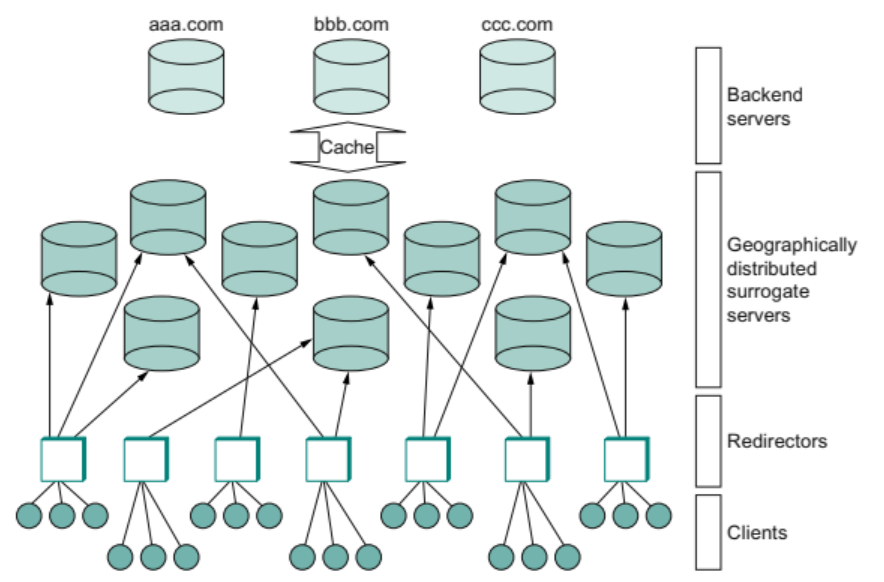
\includegraphics[width=0.8\textwidth
]{images/cdn-distribution.png}
	\caption[CDN]{CDN}
	\label{fig:cdn-distribution}
\end{figure}
Las CDN también necesitan proporcionar un conjunto de redireccionadores que reenvíen las solicitudes de los clientes al servidor más apropiado. El objetivo principal de los redireccionadores es seleccionar el servidor para cada solicitud que resulte en el mejor tiempo de respuesta para el cliente. Un objetivo secundario es que el sistema en su conjunto procese tantas solicitudes por segundo como el hardware subyacente (enlaces de red y servidores web) pueda admitir. El número promedio de solicitudes que se pueden satisfacer en un período de tiempo determinado, conocido como el rendimiento del sistema, es principalmente un problema cuando el sistema está bajo una carga pesada.

\subsubsection{CDNs Comerciales}
Las CDN comerciales usan una combinación de reescritura de URL y redirección basada en DNS. Por razones de escalabilidad, el servidor DNS de alto nivel primero apunta a un servidor DNS de nivel regional, que responde con la dirección real del servidor. Para responder a los cambios rápidamente, los servidores DNS ajustan el TTL de los registros de recursos que devuelven a un período muy corto, como 20 segundos. Esto es necesario para que los clientes no almacenen en caché los resultados y, por lo tanto, no vuelvan al servidor DNS para obtener el último mapeo de URL a servidor.
